\documentclass[11pt]{article}
\usepackage[margin=1in]{geometry}
\usepackage[T1]{fontenc}
\usepackage[utf8]{inputenc}
\usepackage{lmodern}
\usepackage{amsmath,amssymb,amsthm,mathtools}
\usepackage{graphicx}
\usepackage{hyperref}
\usepackage{enumitem}
\usepackage{xcolor}
\usepackage{booktabs}
\usepackage{caption}
\usepackage{float}
\hypersetup{colorlinks=true,linkcolor=blue,citecolor=blue,urlcolor=blue}
\newtheorem{theorem}{Theorem}
\newtheorem{proposition}{Proposition}
\newtheorem{definition}{Definition}
\newtheorem{remark}{Remark}
\newcommand{\eps}{\varepsilon}
\newcommand{\Om}{\Omega}
\newcommand{\Kc}{\mathcal K}
\newcommand{\Rread}{\mathcal R}
\title{Boundary Compensation Origin VI:\\ Spectral Admissibility Collapse and Projection Failure in Frustrated Shadow-Gauge Ensembles\\[0.35em]\large Gershgorin Safety Bounds, Horizon-Crossing Statistics, and Finite-Resolution Readout Failure}
\author{A. A. Malachevsky\\Independent researcher\\Boundary Compensation Origin Program (BC-Origin / BC-O)\\ORCID: 0009-0008-6009-3196\\Software repository: \url{https://github.com/AIDevelopersMonster/boundary-compensation}}
\date{Version v0.1.2 review manuscript, June 2026}
\begin{document}
\maketitle

\begin{abstract}
BC-Origin I introduced observable shadows as localized projections of hidden winding generators through closure-selected inverse denominators. BC-Origin II replaced free couplings by structural kernels. BC-Origin III introduced non-factorizable $Z_2$ edge holonomy and frustrated cycles. BC-Origin IV developed lifted phase-flow and horizon events. BC-Origin V constructed a finite simplicial $Z_2$ shadow-gauge ensemble whose Wilson-like weights arise from spectral trace cycles.

The present paper studies the next question: when does a hidden holonomy configuration fail to produce a localized observable shadow? For each holonomy configuration $\eps$, define
\[
D_\eps=\Delta+\eta A_\eps,
\]
where $\Delta=\operatorname{diag}(d_1,\ldots,d_N)$ is the diagonal closure-denominator strength and $(A_\eps)_{ij}=\eps_{ij}K_{ij}$ is the holonomy-weighted structural adjacency operator. A local shadow branch is admissible only while its eigen-denominator remains above a finite-resolution threshold $\delta$.

The v0.1.2 correction is narrative and structural. It preserves the v0.1.1 ensemble-driven architecture, clarifies the finite-resolution meaning of $\delta$, explains the scalar-diagonal idealization, and integrates the software figures into the mathematical development rather than leaving them as a detached gallery. Frustration is not introduced through an external random sign ratio. Holonomy configurations are distributed according to the BC-Origin V ensemble
\[
Z(\gamma)=\sum_\eps \exp\left(\sum_{\triangle\in F_2}\beta_\triangle(\gamma)\Omega_\triangle\right),
\qquad
\beta_\triangle(\gamma)=6\gamma K_{ij}K_{jk}K_{ki}.
\]
Frustration density is measured from this ensemble rather than imposed by hand.

The paper defines the finite-resolution readout set $\Rread_\delta(D_\eps)=\{a: \lambda_a(D_\eps)>\delta\}$ and identifies projection failure with $\lambda_{\min}(D_\eps)\le\delta$. A Gershgorin safety theorem gives a uniform sufficient condition for all holonomy configurations to remain admissible, while Rayleigh quotients provide sufficient conditions for actual horizon crossing. For $\Delta=d_0I$, the collapse condition is exact:
\[
\lambda_{\min}(D_\eps)=d_0+\eta\lambda_{\min}(A_\eps).
\]
The ensemble then induces the projection-failure observable
\[
P_{\rm fail}(\gamma,\delta)=\left\langle\mathbf 1_{\lambda_{\min}(D_\eps)\le\delta}\right\rangle_\gamma.
\]
The controlled claim is finite-dimensional: within the BC-Origin model, the shadow-gauge ensemble induces a distribution of spectral readout margins, and some regimes produce finite-resolution projection failure. The paper does not claim physical particle annihilation, empirical vacuum ontology, direct Godel incompleteness, or continuum quantum field theory.
\end{abstract}

\section{Introduction}
BC-Origin V supplied the statistical bridge missing from a purely kinematic holonomy model. Edge signs are not arbitrary decorations; they are holonomy configurations in a finite simplicial $Z_2$ shadow-gauge ensemble. The present paper asks how that ensemble affects the spectral viability of localized observable shadows.

The core chain is
\[
Z(\gamma) \longrightarrow \eps \longrightarrow D_\eps \longrightarrow \lambda_{\min}(D_\eps) \longrightarrow \text{readout success or failure}.
\]
The novelty is not merely that Wilson-like loops can be diagnosed. The novelty is that the same holonomy configurations also control the spectral margin of the shadow-readout operator. When that margin crosses a finite-resolution threshold, a hidden configuration may remain algebraically well-defined while failing to return a localized observable shadow.

Figure~\ref{fig:hidden_graph_lab} gives the visual laboratory version of this pipeline: the hidden two-complex, face holonomies, sampled edge signs, and readout status are all displayed as parts of one finite-dimensional calculation.

\begin{figure}[H]
\centering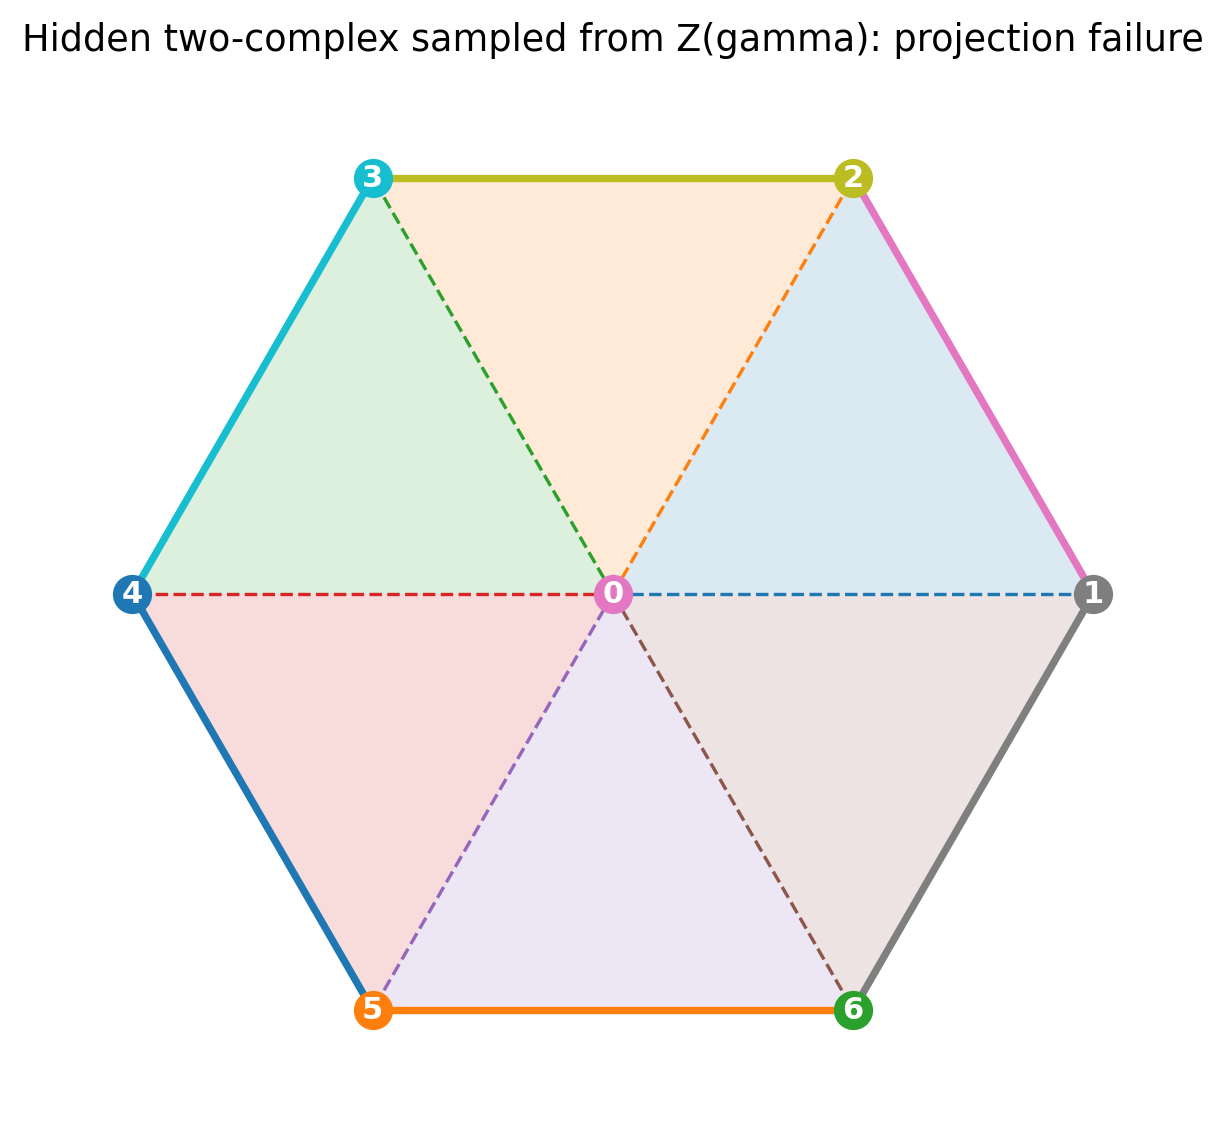
\includegraphics[width=0.72\linewidth]{../origin_vi/figures/hidden_graph_projection_failure_lab.png}
\caption{Hidden structural two-complex sampled from the BC-Origin V ensemble. Edge holonomies and triangular frustrations feed into the shadow-readout operator and its projection-failure status.}
\label{fig:hidden_graph_lab}
\end{figure}

The phrase ``projection failure'' is used in this narrow finite-dimensional sense. It is not a claim that a physical particle is destroyed. It is a statement about the domain of a declared readout protocol.

\section{Internal program context}
The article is self-contained but uses the BC-Origin sequence as its mathematical base. BC-Origin I introduced closure-selected denominators and the admissibility horizon. BC-Origin II introduced deterministic structural kernels. BC-Origin III introduced non-factorizable edge holonomy. BC-Origin IV treated horizon events under lifted phase flow. BC-Origin V introduced the finite simplicial $Z_2$ shadow-gauge ensemble.

The broader Boundary Compensation certification infrastructure is also relevant. BC-XIX--BC-XXII developed a finite-resolution language of thresholded access, dictionary tubes, certificate failure, wall crossing, and no silent continuation. The present paper does not depend on those modules for proof. It uses them as an internal methodological precedent: when a threshold certificate fails, continuation of a local readout object is not assumed silently.

\section{Hidden structural two-complex and ensemble}
\begin{definition}[Hidden structural two-complex]
A BC-Origin VI structural background is a finite object
\[
\Kc=(V,E,F_2,n,K),
\]
where $V$ is a finite vertex set, $E$ is a finite undirected edge set, $F_2$ is a declared set of triangular two-cells, $n_i\in\mathbb Z\setminus\{0\}$ is a hidden winding label, and $K_{ij}=K(n_i,n_j)\ge0$ is a deterministic structural kernel on edges.
\end{definition}

Each edge carries a holonomy variable
\[
\eps_{ij}\in\{-1,+1\}.
\]
For a triangular face $\triangle=(ijk)$, define
\[
\Omega_\triangle=\eps_{ij}\eps_{jk}\eps_{ki}.
\]
BC-Origin V assigns the ensemble weight
\[
w_\gamma(\eps)=\exp\left(\sum_{\triangle\in F_2}\beta_\triangle(\gamma)\Omega_\triangle\right),
\]
with
\[
\beta_\triangle(\gamma)=6\gamma K_{ij}K_{jk}K_{ki}.
\]
The expectation of an observable $F$ is
\[
\langle F\rangle_\gamma=\frac{1}{Z(\gamma)}\sum_\eps F(\eps)w_\gamma(\eps).
\]
Figure~\ref{fig:ensemble_flow} illustrates the resulting ensemble-level diagnostic chain used in the software companion.

\begin{figure}[H]
\centering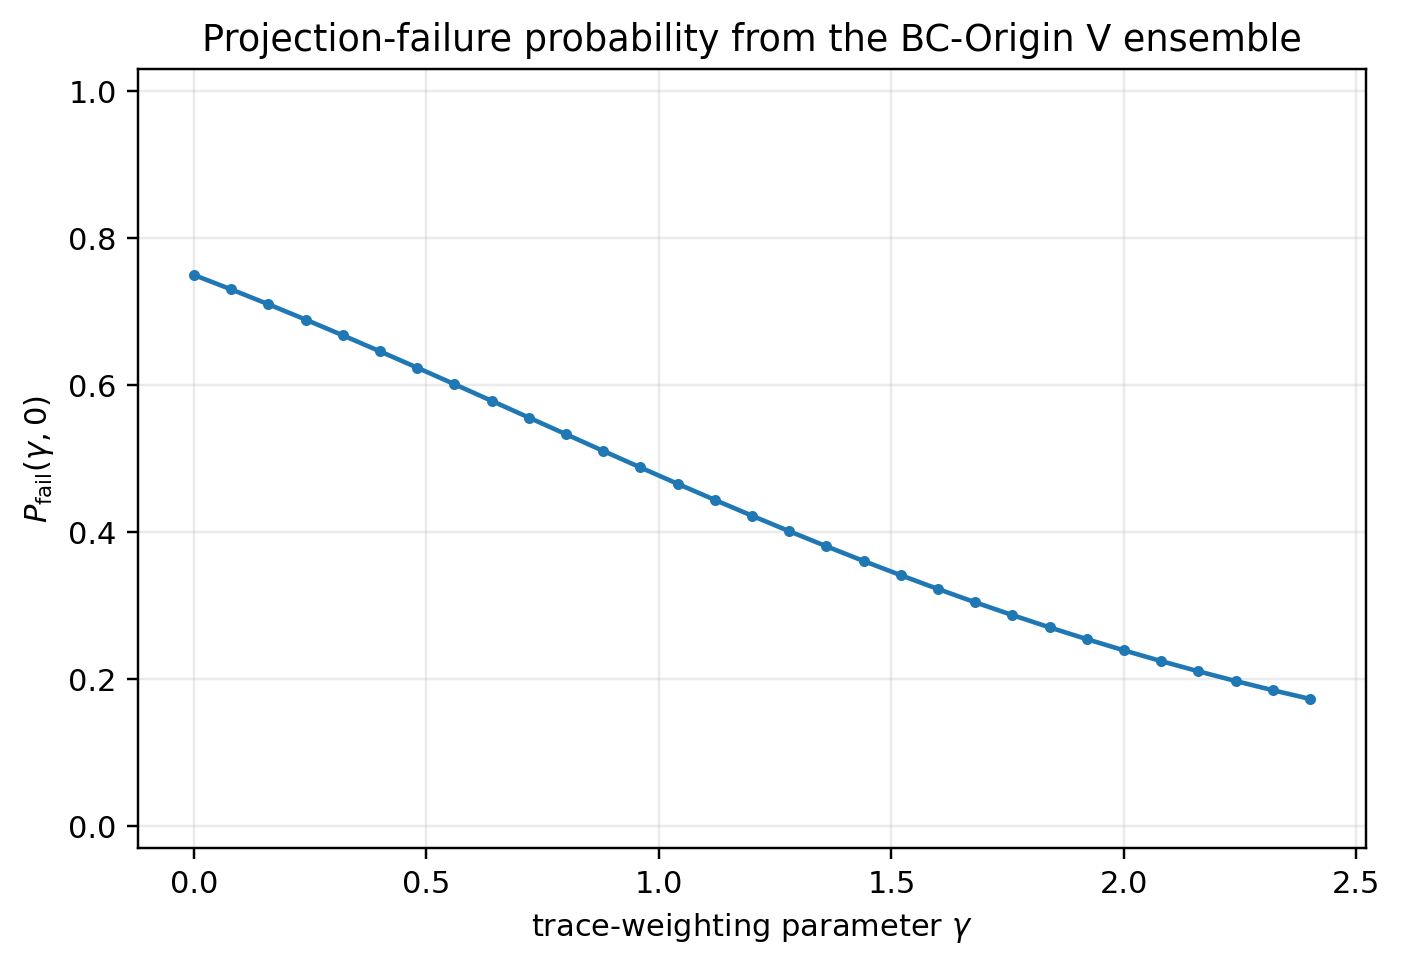
\includegraphics[width=0.82\linewidth]{../origin_vi/figures/p_fail_vs_gamma.png}
\caption{Projection-failure probability induced by the BC-Origin V ensemble. The control parameter is $\gamma$, not an externally prescribed random sign ratio.}
\label{fig:ensemble_flow}
\end{figure}

\section{Shadow-readout operator and finite resolution}
Define
\[
(A_\eps)_{ii}=0,\qquad (A_\eps)_{ij}=\eps_{ij}K_{ij}.
\]
The full readout operator is
\[
D_\eps=\Delta+\eta A_\eps,
\qquad \Delta=\operatorname{diag}(d_1,\ldots,d_N),\quad d_i>0.
\]
Here $\eta$ is a global structural-overlap scale. It is not a physical time parameter and not an empirical coupling constant.

\begin{definition}[Finite-resolution readout set]
For a declared threshold $\delta\ge0$,
\[
\Rread_\delta(D_\eps)=\{a:\lambda_a(D_\eps)>\delta\}.
\]
Projection failure occurs when
\[
\lambda_{\min}(D_\eps)\le\delta.
\]
\end{definition}

The threshold $\delta\ge0$ represents finite readout resolution rather than a new physical constant. In the ideal mathematical limit one may set $\delta=0$, but a macroscopic or finite-resolution observer cannot distinguish arbitrarily small positive denominators from horizon contact. Thus $\lambda_a(D_\eps)\le\delta$ means that the corresponding branch has left the declared resolution domain of the shadow-readout protocol.

Figure~\ref{fig:lambda_distribution} shows how the ensemble produces a distribution of lowest readout eigenvalues rather than a single deterministic margin.

\begin{figure}[H]
\centering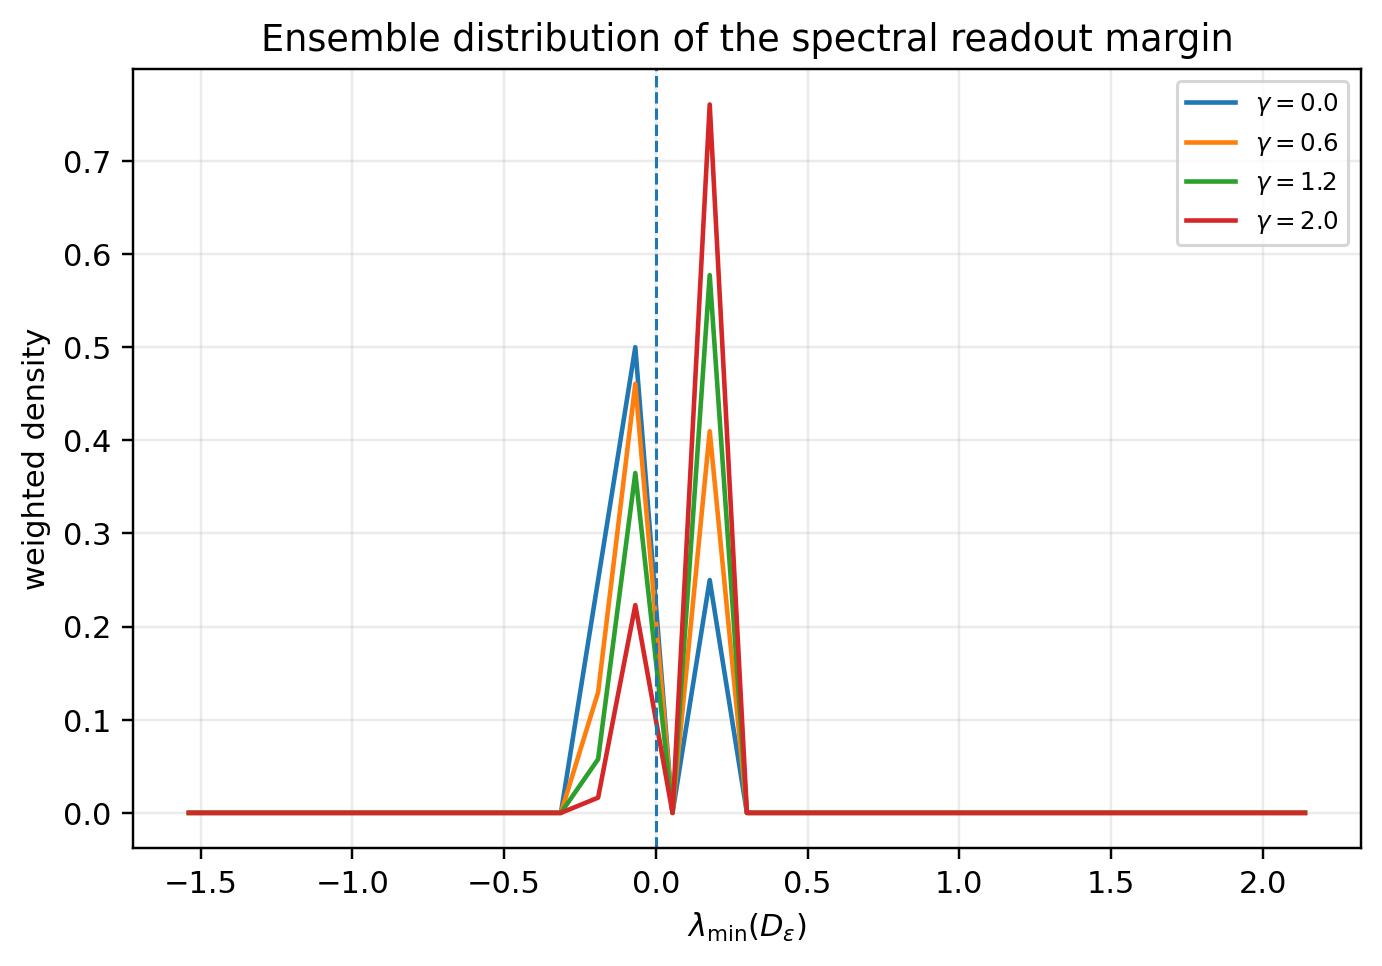
\includegraphics[width=0.82\linewidth]{../origin_vi/figures/lambda_min_distribution_vs_gamma.png}
\caption{The ensemble induces a distribution of spectral readout margins. Threshold crossing is therefore naturally represented as an ensemble-level probability.}
\label{fig:lambda_distribution}
\end{figure}

\section{Measured frustration, not imposed sign disorder}
The v0.1.2 architecture keeps the v0.1.1 correction: it removes the external sign-ratio control. Frustration is not prescribed by a parameter called a random frustration ratio. It is measured from the ensemble:
\[
\Phi(\eps)=\frac12\left(1-\frac{1}{|F_2|}\sum_{\triangle\in F_2}\Omega_\triangle\right).
\]
Thus $\Phi=0$ means all declared triangular faces are balanced, while $\Phi=1$ means all declared triangular faces are frustrated.

The central diagnostics are not functions of a hand-set sign probability. They are ensemble observables:
\[
\langle\Phi\rangle_\gamma,
\qquad
\langle\lambda_{\min}(D_\eps)\rangle_\gamma,
\qquad
P_{\rm fail}(\gamma,\delta).
\]
As demonstrated in Figure~\ref{fig:frustration_gamma}, the measured frustration density is induced indirectly by $\gamma$ through the BC-Origin V ensemble.

\begin{figure}[H]
\centering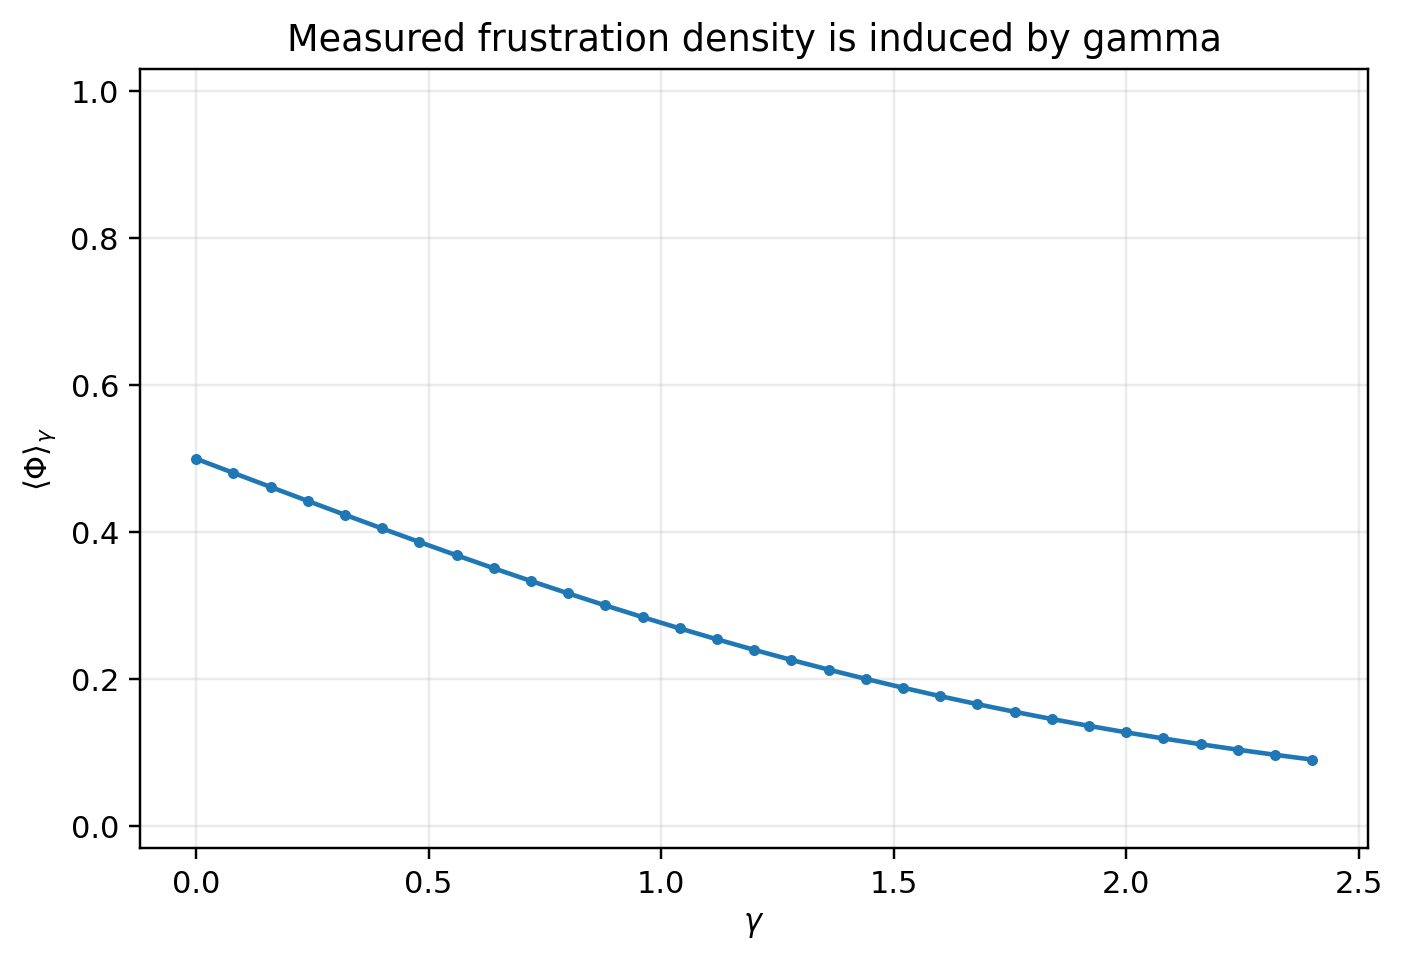
\includegraphics[width=0.82\linewidth]{../origin_vi/figures/frustration_density_vs_gamma.png}
\caption{Frustration density is measured from the ensemble and controlled indirectly by $\gamma$. It is not imposed through an external sign-ratio slider.}
\label{fig:frustration_gamma}
\end{figure}

\section{Gershgorin safety theorem}
\begin{theorem}[Uniform Gershgorin projection-safety criterion]
Let
\[
R_i=\eta\sum_{j\ne i}K_{ij}.
\]
If
\[
d_i-R_i>\delta\qquad\text{for all }i,
\]
then
\[
\lambda_{\min}(D_\eps)>\delta
\]
for every holonomy configuration $\eps$.
\end{theorem}

\begin{proof}
For every row of $D_\eps$, the diagonal center is $d_i$ and the sum of absolute off-diagonal entries is $R_i$. Gershgorin's theorem places every eigenvalue in the union of intervals $[d_i-R_i,d_i+R_i]$. If every lower endpoint is greater than $\delta$, then every eigenvalue is greater than $\delta$ for every sign configuration.
\end{proof}

This theorem is a safety certificate. It does not say that failure of the inequality proves collapse. It says that diagonal dominance is sufficient for uniform readout safety. The difference between a Gershgorin certificate and the actual spectral failure probability is visualized in Figure~\ref{fig:gershgorin_spectral}.

\begin{figure}[H]
\centering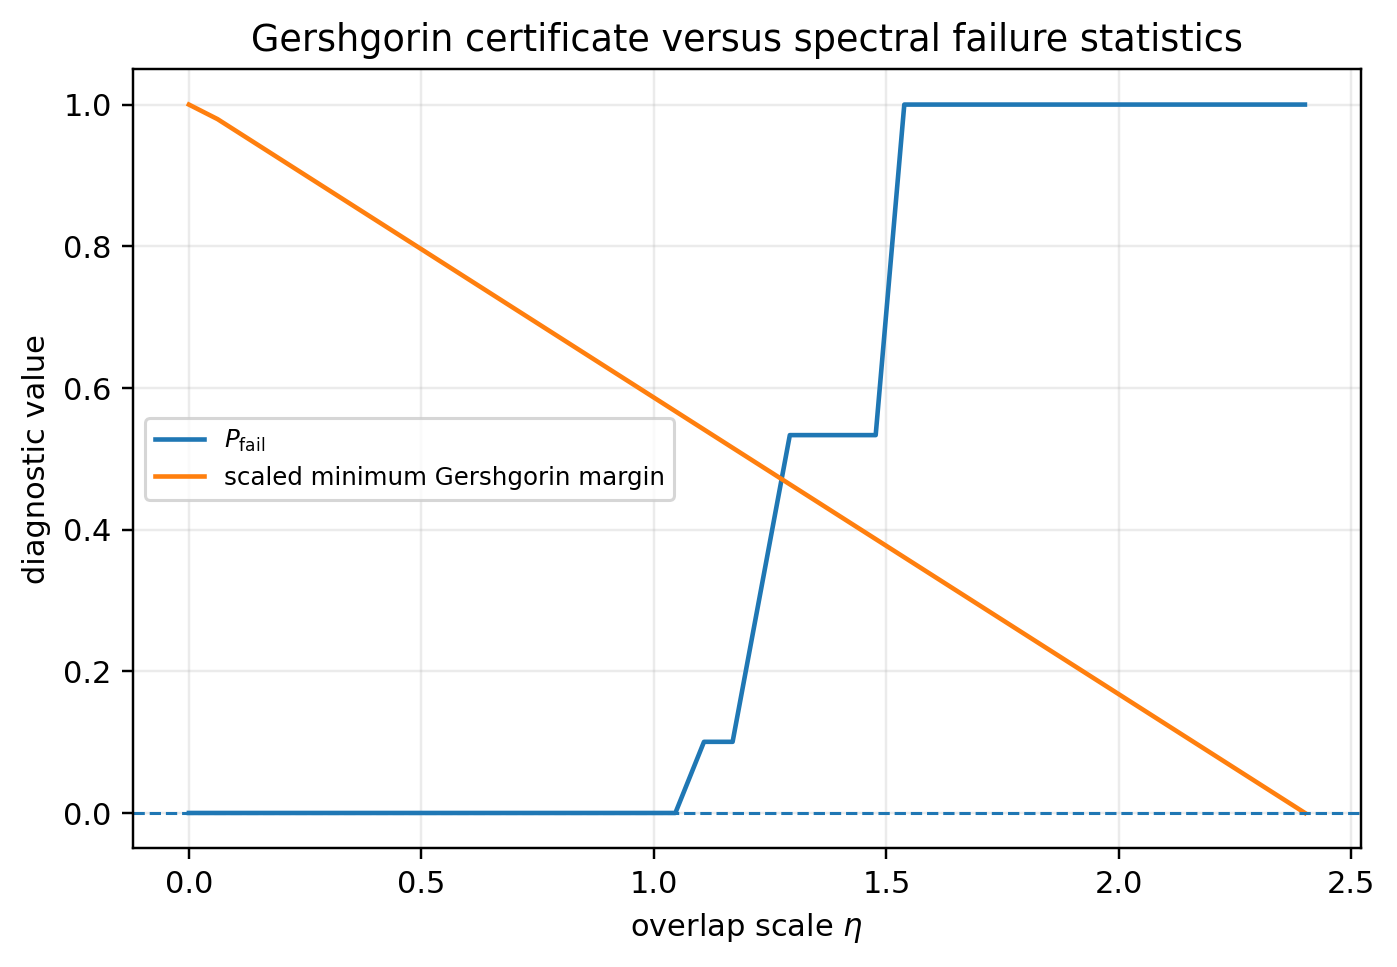
\includegraphics[width=0.82\linewidth]{../origin_vi/figures/gershgorin_vs_spectral_margin.png}
\caption{Gershgorin safety is a certificate; spectral failure is an ensemble event. Loss of the certificate is not automatically a collapse theorem.}
\label{fig:gershgorin_spectral}
\end{figure}

\section{Certificate failure versus actual collapse}
If for at least one vertex
\[
d_i-R_i\le\delta,
\]
then the Gershgorin safety certificate fails. This means uniform safety is no longer certified. It does not mean that $D_\eps$ has crossed the horizon.

This distinction mirrors the finite-resolution certification discipline of the broader BC infrastructure: failure of a certificate is not silently converted into a positive claim. Actual collapse requires an eigenvalue or Rayleigh argument.

\section{Rayleigh collapse criterion}
\begin{theorem}[Rayleigh horizon-crossing criterion]
If there exists $x\ne0$ such that
\[
x^TD_\eps x\le \delta\|x\|^2,
\]
then
\[
\lambda_{\min}(D_\eps)\le\delta.
\]
\end{theorem}

\begin{proof}
By the Rayleigh-Ritz variational characterization,
\[
\lambda_{\min}(D_\eps)=\min_{x\ne0}\frac{x^TD_\eps x}{x^Tx}.
\]
The assumed vector gives an admissible test value at or below $\delta$.
\end{proof}

Figure~\ref{fig:frustration_lambda} illustrates why the paper treats frustration as an ensemble diagnostic rather than as an externally prescribed ratio: the relevant object is the joint distribution of frustration density and spectral margin.

\begin{figure}[H]
\centering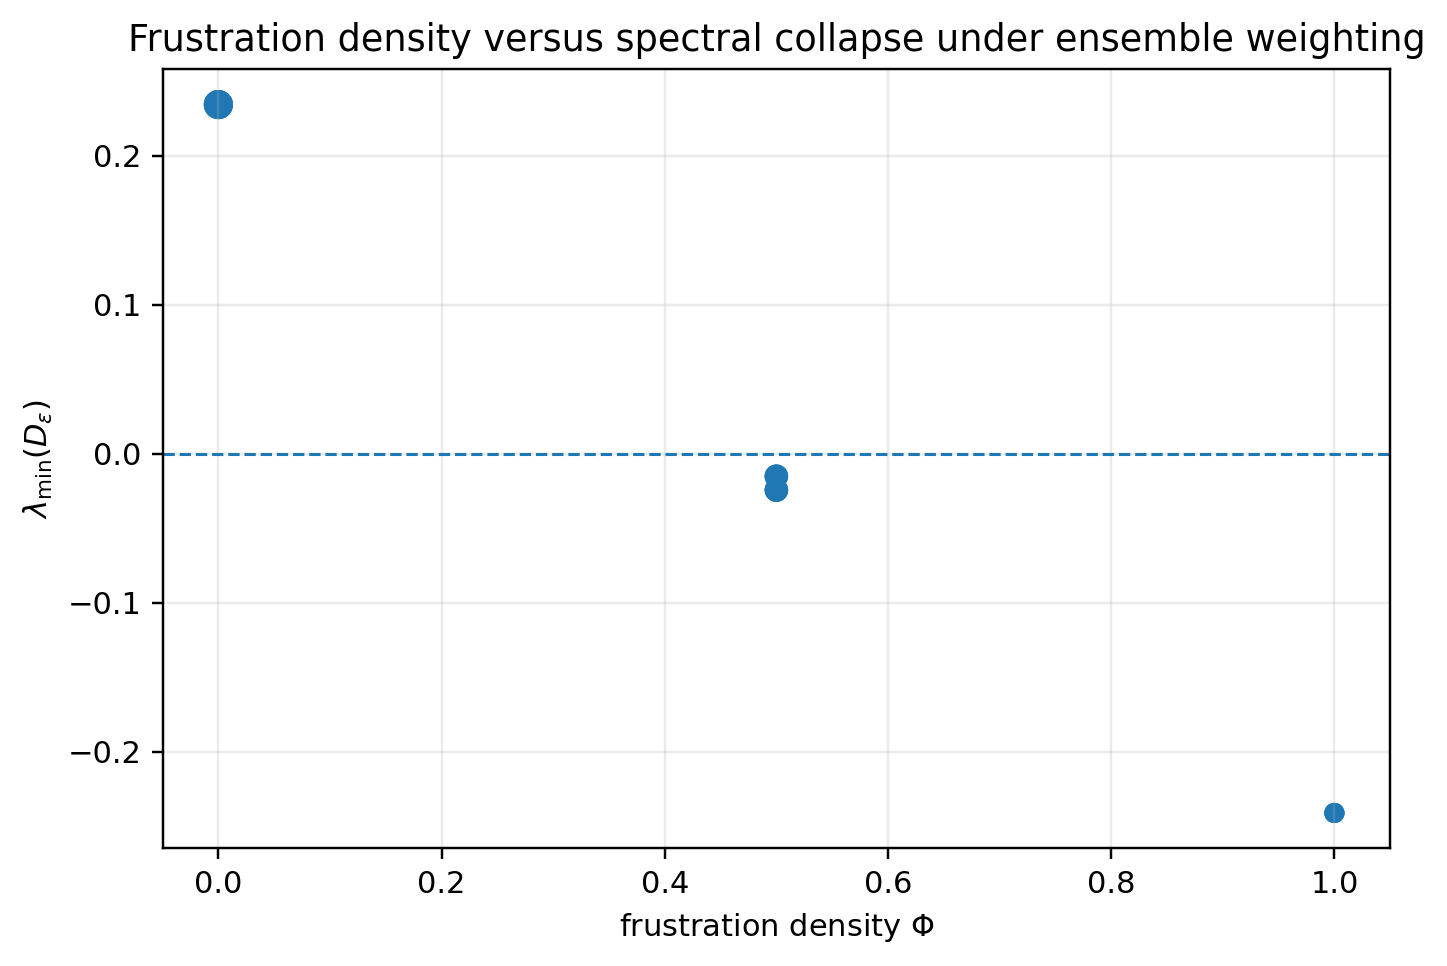
\includegraphics[width=0.82\linewidth]{../origin_vi/figures/frustration_vs_lambda_min_ensemble.png}
\caption{Frustration density versus lowest readout eigenvalue under ensemble weighting. The paper studies this relationship diagnostically rather than asserting a universal equivalence theorem.}
\label{fig:frustration_lambda}
\end{figure}

\section{Exact scalar-diagonal collapse}
The scalar-diagonal case $\Delta=d_0 I$ represents a homogeneous closure background: before holonomy coupling is switched on, all hidden shadow branches have the same denominator strength. This idealization is not generic, but it isolates the exact role of the holonomy-weighted adjacency spectrum.

When $\Delta=d_0I$,
\[
D_\eps=d_0I+\eta A_\eps.
\]
Therefore
\[
\lambda_{\min}(D_\eps)=d_0+\eta\lambda_{\min}(A_\eps).
\]
Projection failure is exactly
\[
d_0+\eta\lambda_{\min}(A_\eps)\le\delta.
\]
In this minimal case, BC-Origin VI has a sharp collapse criterion rather than only a safety bound. The corresponding exact boundary is shown in Figure~\ref{fig:scalar_boundary}.

\begin{figure}[H]
\centering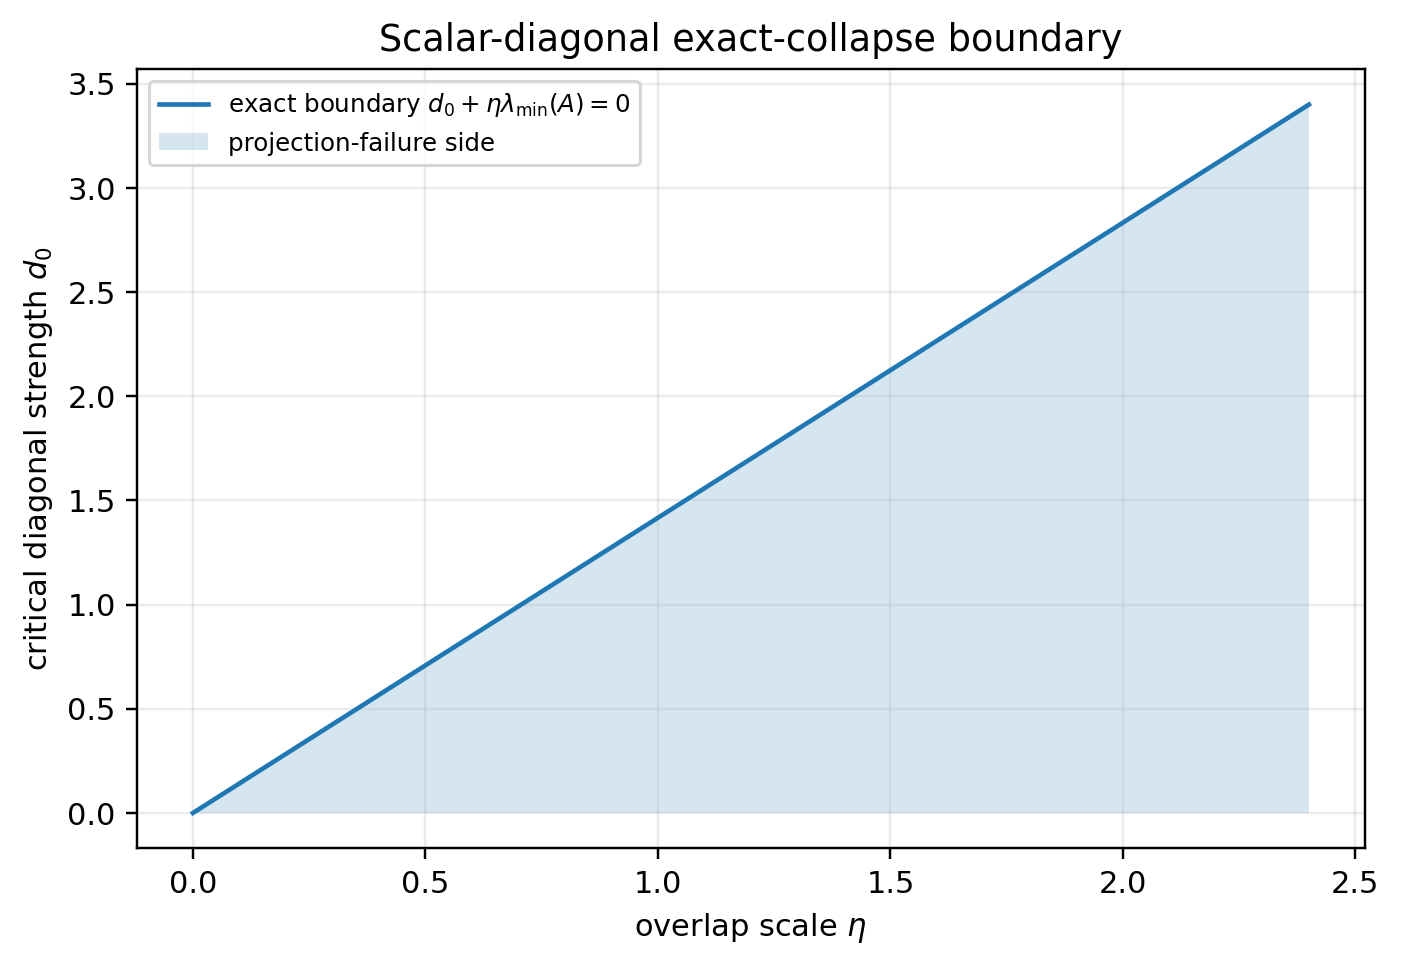
\includegraphics[width=0.82\linewidth]{../origin_vi/figures/scalar_diagonal_collapse_boundary.png}
\caption{Scalar-diagonal exact-collapse boundary. In this homogeneous closure background, the collapse condition is controlled directly by the lowest eigenvalue of $A_\eps$.}
\label{fig:scalar_boundary}
\end{figure}

\section{Ensemble-induced projection failure}
\begin{definition}[Projection-failure probability]
The BC-Origin V ensemble induces
\[
P_{\rm fail}(\gamma,\delta)=\left\langle\mathbf 1_{\lambda_{\min}(D_\eps)\le\delta}\right\rangle_\gamma.
\]
The complementary admissibility probability is
\[
P_{\rm adm}(\gamma,\delta)=1-P_{\rm fail}(\gamma,\delta).
\]
\end{definition}

For the scalar-diagonal case,
\[
P_{\rm fail}(\gamma,\delta)=\Pr_{\eps\sim Z(\gamma)}[d_0+\eta\lambda_{\min}(A_\eps)\le\delta].
\]
This is the central formula of the paper. Figure~\ref{fig:ensemble_flow} showed the resulting $P_{\rm fail}$ curve, while Figure~\ref{fig:lambda_distribution} showed the underlying spectral-margin distribution.

\section{Wilson-loop background and spectral-collapse foreground}
BC-Origin V made Wilson-like cycle diagnostics available. BC-Origin VI does not replace them; it adds a distinct observable. Wilson loops diagnose gauge-cycle order. The spectral margin diagnoses readout viability.

The proper bridge is
\[
\text{gauge ensemble}\to\text{holonomy statistics}\to\text{spectral margin distribution}\to\text{projection-failure probability}.
\]
It is not claimed that loss of a Wilson area law is mathematically equivalent to projection failure in all finite complexes. The controlled claim is that both are observables of the same ensemble and can be compared. Figure~\ref{fig:wilson_projection} compares these related but distinct diagnostics.

\begin{figure}[H]
\centering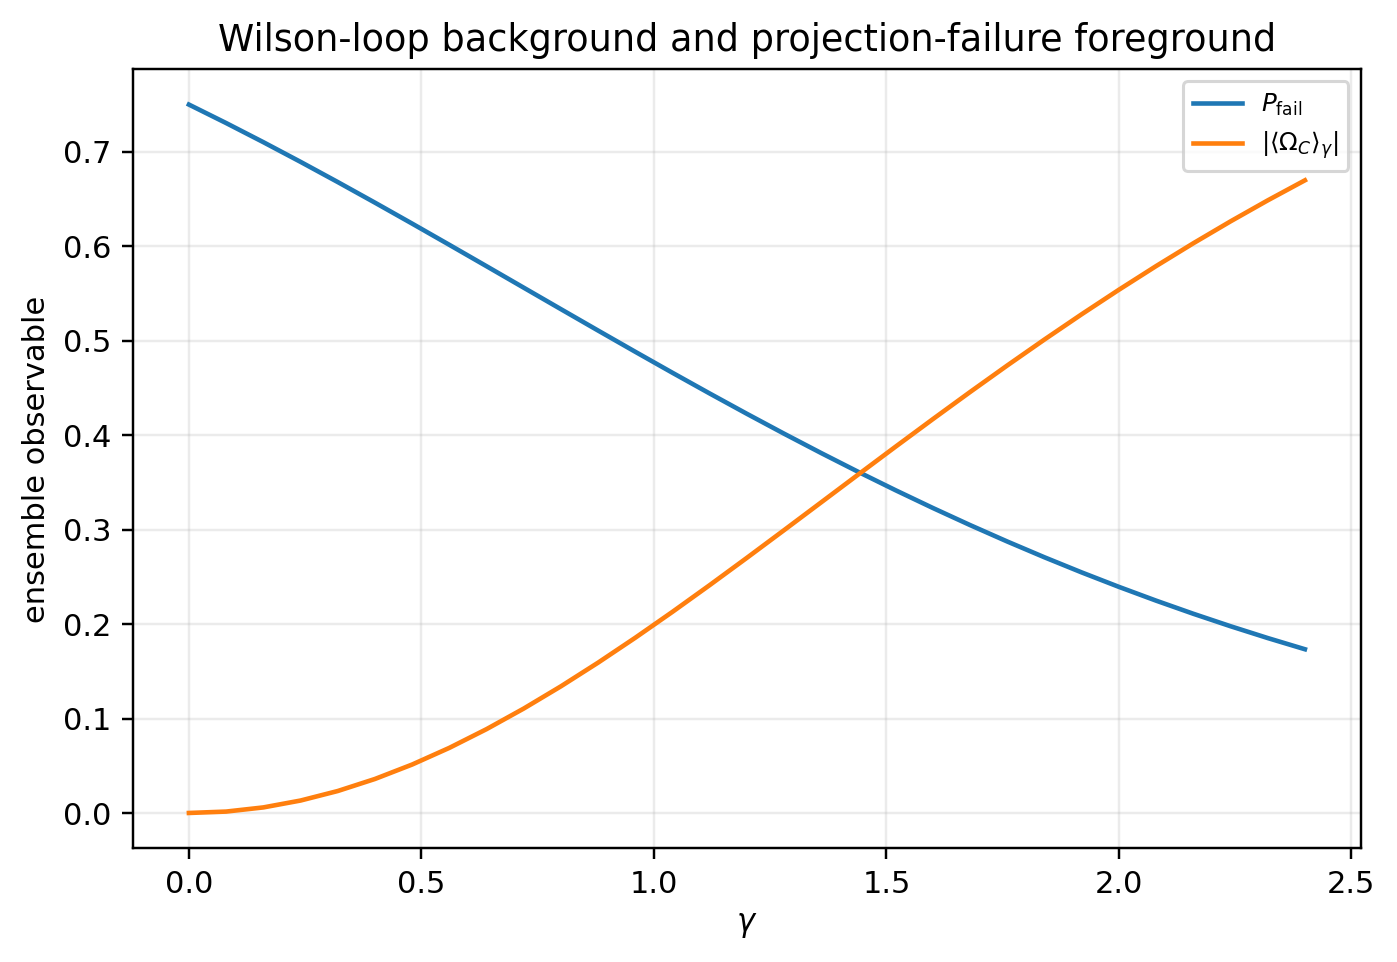
\includegraphics[width=0.82\linewidth]{../origin_vi/figures/wilson_loop_vs_projection_failure.png}
\caption{Wilson-loop diagnostics provide a gauge-ensemble background; projection failure is the spectral-readout foreground. The two observables are comparable but not identical.}
\label{fig:wilson_projection}
\end{figure}

\section{Software companion and validation}
The software package follows the corrected ensemble-driven architecture. Its core functions enumerate or sample holonomy configurations from $Z(\gamma)$, compute $D_\eps$, compute $\lambda_{\min}$, compute $P_{\rm fail}$, and compare exact enumeration with MCMC on small complexes.

For small complexes, exact enumeration is used to validate the MCMC sampler; see Figure~\ref{fig:exact_mcmc}. Figure~\ref{fig:mcmc_trace} gives a basic trajectory diagnostic for sampled frustration and spectral margin.

\begin{figure}[H]
\centering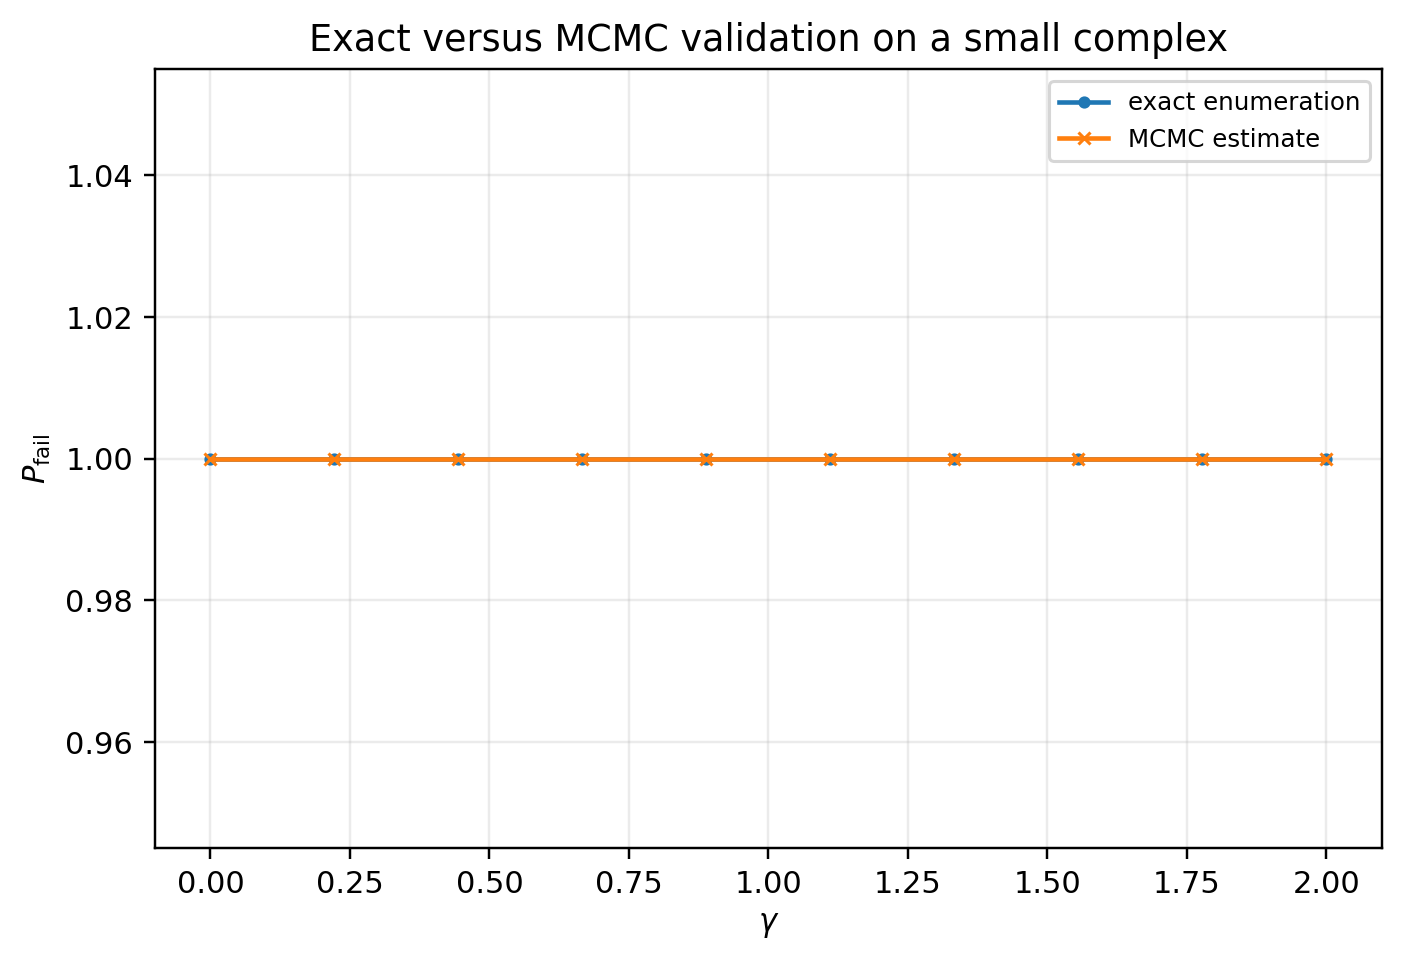
\includegraphics[width=0.82\linewidth]{../origin_vi/figures/exact_vs_mcmc_validation.png}
\caption{Exact enumeration and MCMC validation on a small complex. This guards against treating the sampler as a source of uncontrolled numerical evidence.}
\label{fig:exact_mcmc}
\end{figure}

\begin{figure}[H]
\centering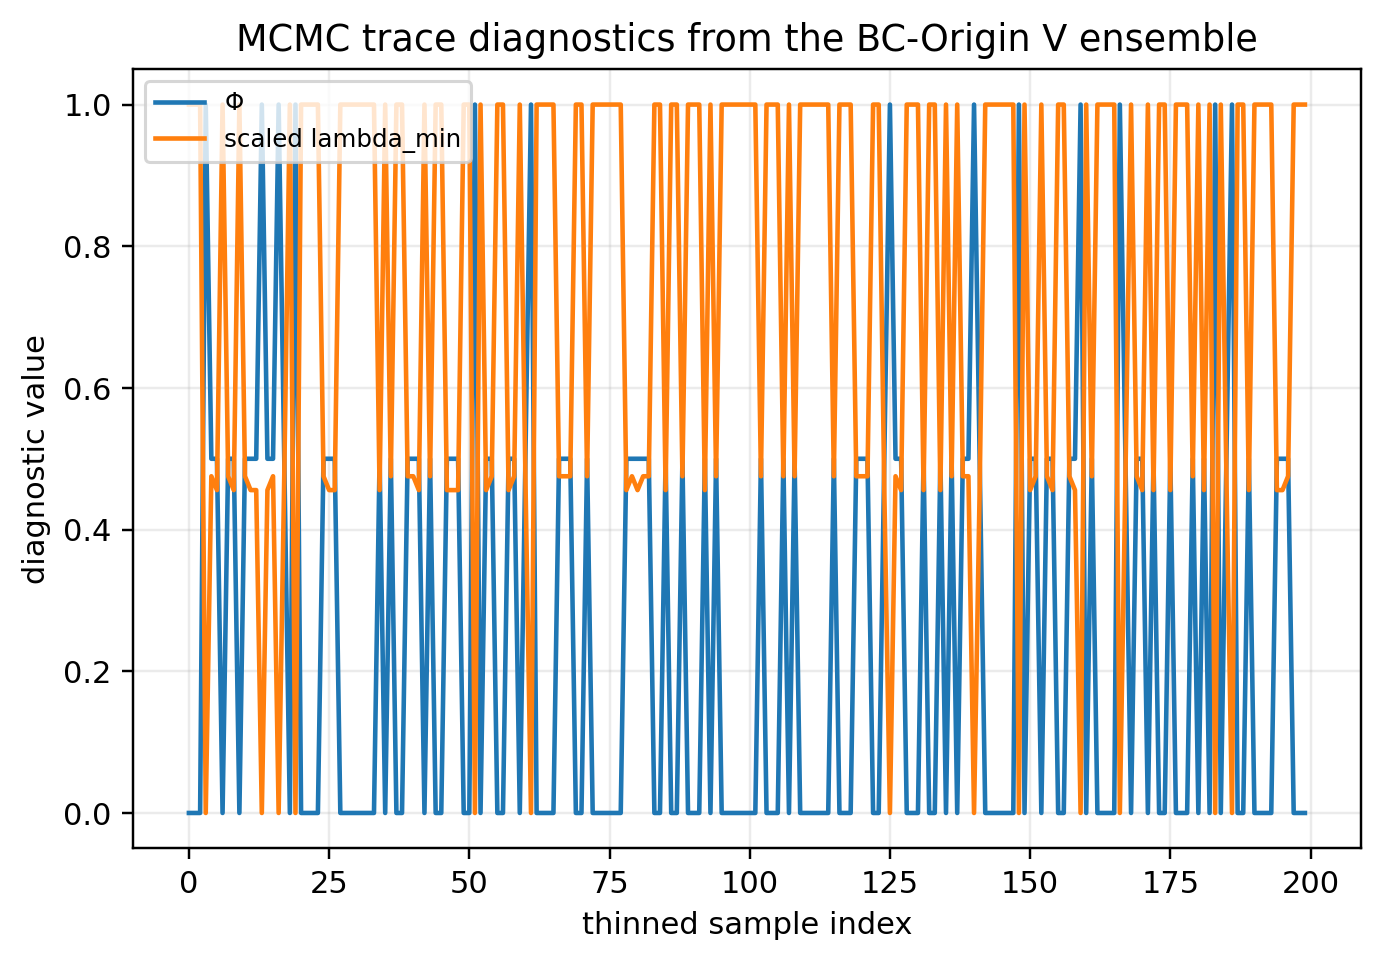
\includegraphics[width=0.82\linewidth]{../origin_vi/figures/mcmc_trace_diagnostics.png}
\caption{MCMC trace diagnostics from the BC-Origin V ensemble. The trace is a computational diagnostic, not an independent source of physical stochasticity.}
\label{fig:mcmc_trace}
\end{figure}

The package contains:
\begin{itemize}[leftmargin=1.5em]
\item a Python core module for exact enumeration and MCMC sampling;
\item a figure generator;
\item a browser-based HTML lab;
\item JSON examples of a single triangle, two triangles sharing an edge, and a triangulated disk;
\item bibliographic and Zenodo metadata drafts;
\item no-formula article descriptions in English and Russian.
\end{itemize}

The software repository pointer is included for continuity:
\[
\text{\url{https://github.com/AIDevelopersMonster/boundary-compensation}}.
\]

\section{Controlled claims}
This paper claims:
\begin{enumerate}[leftmargin=1.5em]
\item finite-resolution shadow readout can be formalized by $\Rread_\delta(D_\eps)$;
\item $\delta$ encodes finite readout resolution rather than a new physical constant;
\item BC-Origin V induces a distribution of holonomy configurations through $Z(\gamma)$;
\item frustration density is measured from that ensemble, not imposed by a sign-ratio parameter;
\item Gershgorin diagonal dominance gives a uniform projection-safety certificate;
\item loss of that certificate is not identical to actual collapse;
\item Rayleigh quotients provide sufficient collapse criteria;
\item the scalar-diagonal case admits an exact collapse condition;
\item $P_{\rm fail}(\gamma,\delta)$ is a well-defined finite-ensemble observable;
\item Wilson-loop diagnostics and spectral projection-failure diagnostics are related ensemble observables, but no universal equivalence is claimed.
\end{enumerate}

\section{Non-claims}
The paper does not claim physical particle annihilation, empirical vacuum dynamics, direct Godel incompleteness, continuum lattice QFT, QCD confinement, Standard Model dynamics, quantum measurement collapse, or destruction of hidden structure. It gives a finite-dimensional model of readout-domain failure.

\section{Conclusion}
BC-Origin VI shifts attention from gauge-cycle weights alone to the spectral viability of localized shadows. The corrected architecture uses the BC-Origin V ensemble as the source of holonomy statistics. This makes projection failure an ensemble-induced spectral observable, not a consequence of externally imposed random signs.

A hidden configuration can be algebraically present while failing to produce a localized observable shadow at finite resolution. This is the controlled mathematical content of spectral admissibility collapse.

\begin{thebibliography}{99}
\bibitem{originI} A. A. Malachevsky, \emph{Boundary Compensation Origin I: Oriented Winding Shadows, Structural Scale Selection, and Signed Spectral Localization}, v0.1.1 preprint with software appendix, 2026. Related DOI: \href{https://doi.org/10.5281/zenodo.20822186}{10.5281/zenodo.20822186}.
\bibitem{originII} A. A. Malachevsky, \emph{Boundary Compensation Origin II: Structural Coupling Kernels and Multi-Shadow Spectral Geometry}, v0.1.0 preprint, 2026.
\bibitem{originIII} A. A. Malachevsky, \emph{Boundary Compensation Origin III: Non-Factorizable Holonomy and Frustrated Multi-Shadow Spectral Geometry}, v0.1.1 clean manuscript, 2026.
\bibitem{originIV} A. A. Malachevsky, \emph{Boundary Compensation Origin IV: Lifted Phase Flow, Closure-Lift Spectral Pumping and Horizon Events in Multi-Shadow Geometry}, v0.1.0 manuscript, 2026.
\bibitem{originV} A. A. Malachevsky, \emph{Boundary Compensation Origin V: Simplicial $Z_2$ Shadow-Gauge Ensembles}, v0.1.3 review manuscript, 2026.
\bibitem{bcxix} A. A. Malachevsky, \emph{Boundary Compensation XIX: Algorithmic Construction of Finite-Dimensional Hidden-Lift Dictionaries}, v0.1.1, 2026, DOI: \href{https://doi.org/10.5281/zenodo.20783642}{10.5281/zenodo.20783642}.
\bibitem{bcxx} A. A. Malachevsky, \emph{Boundary Compensation XX: Certified Atlas Transitions for Parameter-Dependent Dictionary Tubes}, v0.1.1, 2026, DOI: \href{https://doi.org/10.5281/zenodo.20786712}{10.5281/zenodo.20786712}.
\bibitem{bcxxii} A. A. Malachevsky, \emph{Boundary Compensation XXII: Metrics and Stability Distances on Thresholded Dictionary Tubes}, v0.1.1, 2026, DOI: \href{https://doi.org/10.5281/zenodo.20790084}{10.5281/zenodo.20790084}.
\bibitem{gershgorin} S. A. Gershgorin, ``Uber die Abgrenzung der Eigenwerte einer Matrix,'' \emph{Izvestiya Akademii Nauk SSSR, Otdelenie fiziko-matematicheskikh nauk}, 1931.
\bibitem{varga} R. S. Varga, \emph{Gersgorin and His Circles}, Springer, 2004.
\bibitem{wilson} K. G. Wilson, ``Confinement of Quarks,'' \emph{Physical Review D} \textbf{10}, 2445--2459, 1974.
\bibitem{wegner} F. J. Wegner, ``Duality in Generalized Ising Models and Phase Transitions without Local Order Parameter,'' \emph{Journal of Mathematical Physics} \textbf{12}, 2259--2272, 1971.
\bibitem{kogut} J. B. Kogut, ``An Introduction to Lattice Gauge Theory and Spin Systems,'' \emph{Reviews of Modern Physics} \textbf{51}, 659--713, 1979.
\bibitem{elitzur} S. Elitzur, ``Impossibility of Spontaneously Breaking Local Symmetries,'' \emph{Physical Review D} \textbf{12}, 3978--3982, 1975.
\bibitem{tropp} J. A. Tropp, ``User-Friendly Tail Bounds for Sums of Random Matrices,'' \emph{Foundations of Computational Mathematics} \textbf{12}, 389--434, 2012; arXiv:1004.4389.
\bibitem{wigner} E. P. Wigner, ``Characteristic Vectors of Bordered Matrices with Infinite Dimensions,'' \emph{Annals of Mathematics} \textbf{62}, 548--564, 1955.
\end{thebibliography}
\end{document}
